\documentclass{article} 
\usepackage{url, graphicx}
\usepackage[margin=1in]{geometry}

\title{Graph and Search Library Design Document}
\author{
Andrew Grant\\
\texttt{amg2215@columbia.edu}
\and 
Anton Igorevich \\
\texttt{ain2108@columbia.edu}
\and
 Somya Vasudevan \\
 \texttt{sv2500@columbia.edu}
}
\date{4/28/2017}

\begin{document}

\maketitle

\section{Introduction}
This is a graph library, built in C++, that makes it easy to create, use and run algorithms on graphs. The library is designed to make it really easy for users to use their own vertex and edge data structures. The user will define his/her Vertex and Edge types and then will immediately be able to start using the library and start running algorithms on graphs. Currently the library supports the following graphs: DG (directed graph), DAG (directed acyclic graph), DT (directed tree), Matrix(undirected). The idea is that users define their own vertex and edge data types, and then the library handles everything else under the hood.

Conceptually, a graph is made up of a bunch of vertices and edges. At a minimum there must be some way to distinguish between vertices, distinguish between edges, and define edges as made up of two vertices. Nonetheless, users often want to embed extra information in these ADTs. For example, a user may want a graph representing cities and the highways between them. The user may have a City class; cities must of course have some unique id (e.g. city name), but they may also have extra information such as population, GDP, etc. The same goes for edges; maybe a Road class is used, and the class also has miles, age of road etc. This library makes it easy for users to provide their own ADTs, and immediately start creating graphs, and run algorithms on them.

\section{Philosophy}
The philosophy of the library was that it should be really easy for users to be able to use their own vertex and edge data structures, and that the the library would handle everything else under the hood. In order to make it easy to use the library, we designed the library with minimal requirements when it came to the user defined vertex and edge types. 

\section{User Defined Vertex and Edge}
The library was designed so that users are able to design their own vertex and edge data structures. All that is required of the users is the following:
\begin{itemize}
\item Vertex and Edge must be comparable (that is they must implement the == operator for their types)
\item Vertex and Edge must be hashable (
\item Edge must have two fields \texttt{v\_1} and \texttt{v\_2}, that are of the same type as the Vertex that they defined.
\item To use the path algorithms, Edge must have a cost field that is numeric. If the user does not define a cost, the library will automatically given an edge a cost of 1.
\item Vertex must have a \texttt{to\_string} function that returns a string representation of the vertex. 
\end{itemize}

\section{General Graph Design}
Because minimal requirements are imposed on the user when it comes to his/her vertex and edge type, we needed to wrap the users data types in our own struct for certain bookkeeping reasons. Thus, under the hood the graph library stores each vertex in a \texttt{vertex\_wrapper}. This wrapper also stores a field of type \texttt{Value} which is a pair consisting of a string and an int. This lets the user set some sort of value for each vertex, which their own data type knowing about such a value. Lastly, the wrapper also stores a unique id (of type int) that the user is again completely oblivious to. This id is generated by the graph library for internal bookkeeping (for example, it's used as the index when a matrix graph representation is used). 
\par
This \texttt{vertex\_wrapper} is the fundamental data type of our graph library. Whether a DAG, DG, DT or matrix graph representation is used, each vertex is stored in this struct. 

\section{Adjacency List Design}
In order to implement an adjacency list, we actually created another data type to wrap \texttt{vertex\_wrapper}, which we call \texttt{vertex\_header}. The \texttt{vertex\_header} is the head of a vertex's adjacent list. Thus, the difference between a \texttt{vertex\_header} and \texttt{vertex\_wrapper}, is that the \texttt{vertex\_header} is the conceptual head of a vertex's adjacency list and points to a list of  \texttt{vertex\_wrapper}.
\newpage

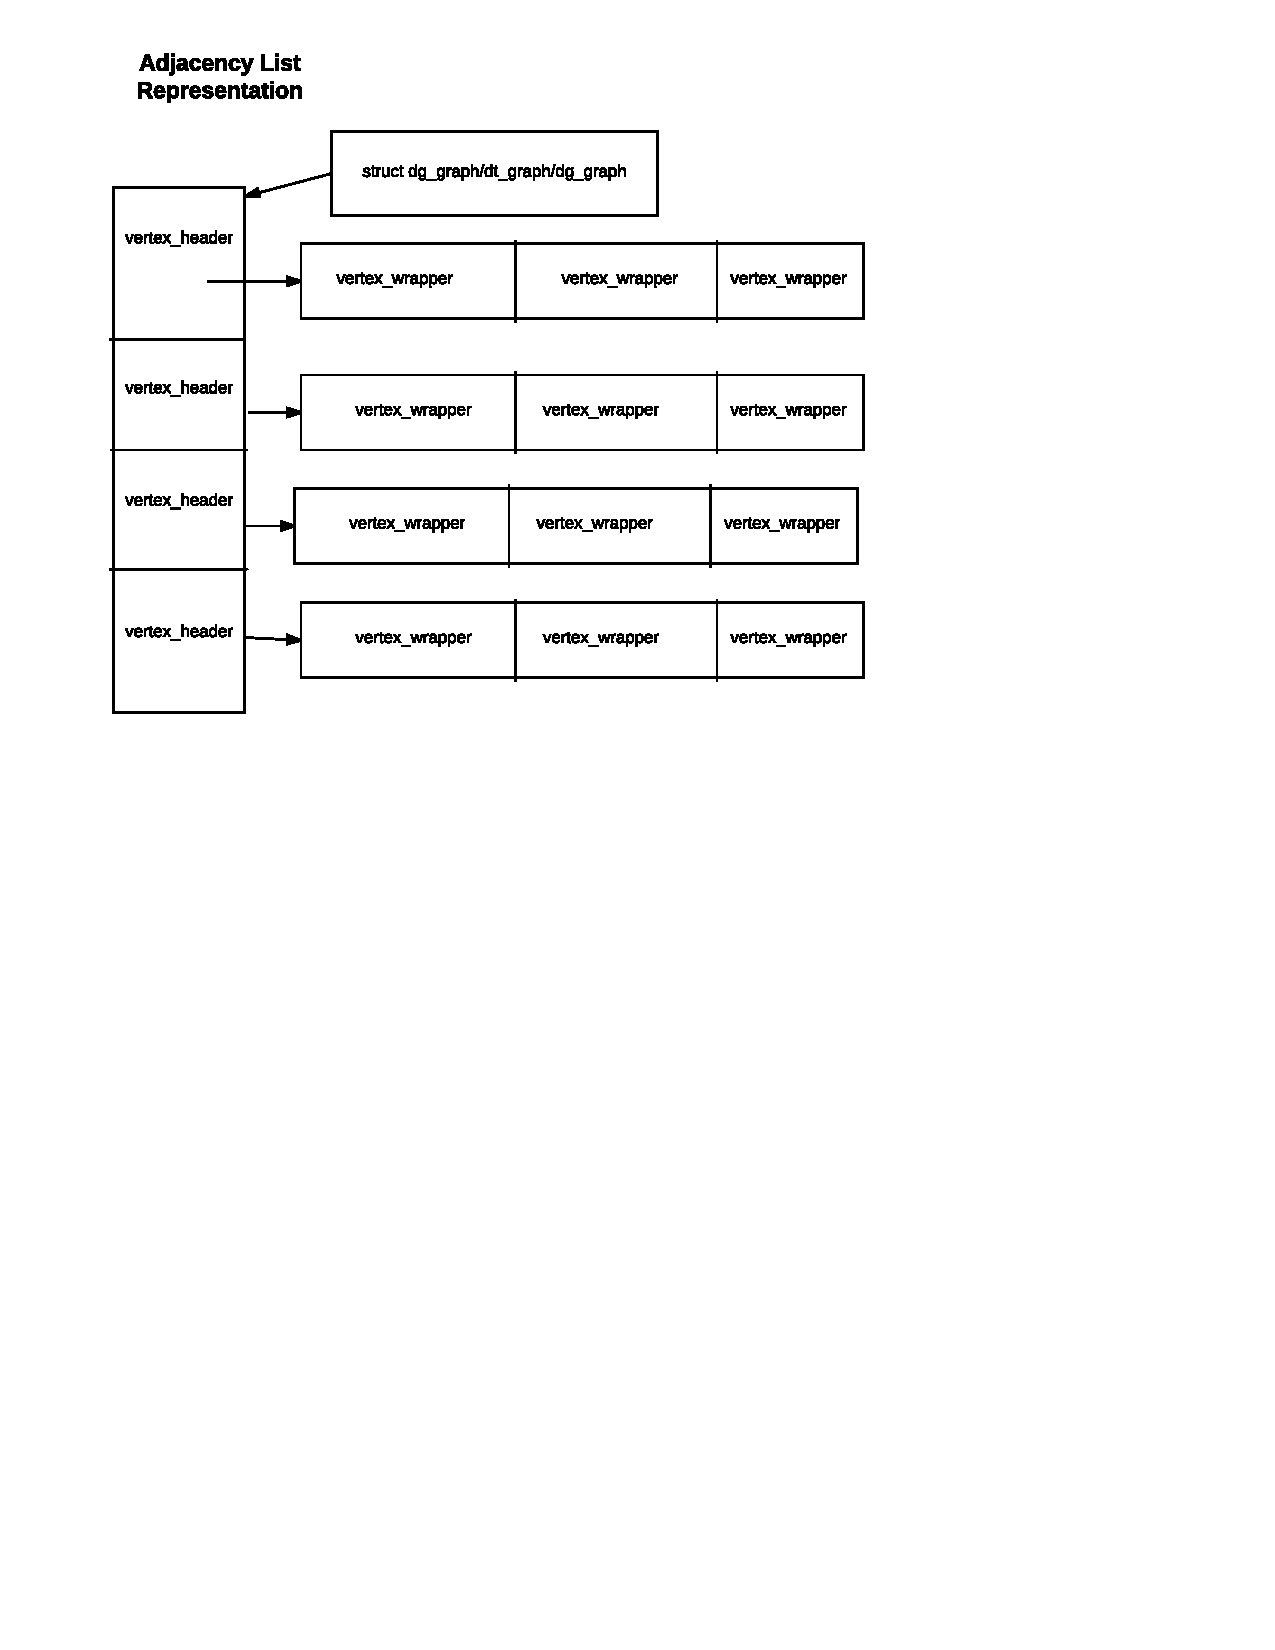
\includegraphics{al}

\newpage

\section{Matrix Design}

\section{Concepts}

Reference: \url{http://www.stroustrup.com/good_concepts.pdf}

Concepts are essentially compile time predicates. That is, they are requirements on the types that are passed into functions. If an argument doesn't satisfy the concept, the compiler will immediately report an error. This makes debugging much easier when using templates. Without concepts, debugging can be very tricky when using templates, as it's often late in the compilation process that the compiler realizes a type is no good. As a result error messages can be extremely long, making dubugging tricky. 

In terms of this library, the idea is that user defined vertices and edges must satisfy certain properties; concepts are used to enforce these. For example, an Edge must point to two vertices; an Edge must be comparable; a Vertex must have a unique identifier. We also use concepts to support function overloading. The names of the functions that work on graphs are all the same; so the user can call the same function whether he or she is working with a matrix or adjacency list. Concepts are used to determine which function should be called.

\section{Conclusion}

\section{Repository Information}
The complete project is located at \url{https://github.com/andyg7/Graph-Library}.
The core graph library code is located at \url{https://github.com/andyg7/Graph-Library/src}

\end{document} 